% Rust
\chapter{Rust - a new system level programming language}

To better understand where Rust, a new system level programming language, is placed among others of its kind, it is necessary to understand the difficulties that can arise by using them. Described by Bjarne Stroustrup, the creator of C++, in his book \textit{'The C++ programming language'}, one purpose of a programming language is to provide "a vehicle for the programmer to specify actions to be executed by the machine". That is even more true for a language that is used to create software that needs to utilize the underlying hardware very well to run at a good performance level. C++, and now Rust, are languages that provide the tools a programmer needs to write code that runs well on the hardware. But because that tools grant great power and control, any error done when implementing an application can be costly and have severe consequences. And there are two problems that, based on history and experience, prove quite difficult to solve. That problems are writing \textit{secure} and/or \textit{multi-threaded} code.
Secure code is often related to memory management and with languages that allow for manually controlling memory operations, the complexity of this issue increases. Consequences of these difficulties are security vulnerabilities and exploits, that also affected bigger companies without mentioning any names.
Although multi-threaded code does not that often cause security holes, the complexity, introduced by its parallel and asynchronous fashion, is the reason for errors that are hard to identify or even reproduce.

Rust tries to solve exactly this issues while claiming to maintain performance similar to the one of C or C++. Rust is developed by Mozilla and an open source community. It allows the programmer to manage the memory used by the application manually and tries to uphold a close relationship between language operations and the machine's hardware. While trying to solve problems that can occur in code written in C++, Rust shares several common principles with it. One of them being the ambition Bjarne Stroustrup has expressed for C++ in his paper \textit{"Abstraction and the C++ Machine Model"}:

\begin{quote}
	In general, C++ implementations obey the zero-overhead principle: What you don’t use, you don’t pay for. And further: What you do use, you couldn’t hand code any better.
\end{quote}

While following this and other principles shared with C++, Rust adds own standards it wants to uphold, including memory safety or simplified and trustworthy concurrency. To meet these promises, Rust relies heavily on compile-time checks that collaborate well with its static type system. 
In statically typed languages, the types of variables are checked at compile-time by a part of the compiler called the type-checker. Because those checks are not performed at the program's runtime, these languages are said to be \textit{statically type checked}. This comes with the advantage of allowing certain runtime checks to be omitted, which removes execution overhead and reduces the binary size. To prevent a common misunderstand when talking about statically typed languages, it has to be mentioned that \textit{type inference} does not prevent static type checking. Type inference is a language feature, that allows the programmer to omit any specific type when declaring a variable. The type is chosen by the compiler based on the context within a variable was declared and by knowing the type of the value that was assigned to it. 

Combined with its novel ownership system, that allows the definition of lifetimes for used values, it ensures memory safety without the need of a garbage collector. A garbage collector is a system that tracks memory allocations at runtime and manages their lifetime instead of the programmer. It is commonly used in higher level languages such as Java or C\#, but the safety comes with a cost in performance. When ownership shall be transfered from one owner to the new one, Rust uses the concept of \textit{moving} and defines \textit{borrows}, that allow temporary usage of values without affecting their ownership. These techniques, which are later described in more details, build the basis for the memory safety in Rust. They also provide the foundation Rust's concurrency model is built upon. Again, by using compile-time checks, Rust is able to detect certain problems related to multi-threaded code before the program is run once. 

This section continues with a description of Rust's current state and its ecosystem, followed a detailed description of the concepts that defined the language. They are explained and illustrated with code examples to built a better understanding. The shown code samples are compared to corresponding ones in C++, to show the difference between those languages.

\section{Language's current state}

With version 1.0 being released in 2014, Rust is a rather young programming language. The current version is 1.25.0, which was shipped on March 29, 2018. Examining the release notes and corresponding dates, it can be observed that about every six weeks a new major version upgrade is released. Version upgrades include \acp{RFC} issued by the community or by dedicated working groups. Another source of feedback for the language comes from the developers of \textit{Servo}, a new web browser engine entirely developed in Rust, which is developed by Mozilla. Servo powers the newest version of the Firefox browser and serves as a real-world test of Rust. Beside the concepts already mentioned above, Rust is embedded into an ecosystem that includes many tools that simplify the live of a developer. The parts of the ecosystem are described in the following section.

\section{Rust ecosystem}

During the development process of Rust several tools, alongside the Rust compiler \textit{rustc}, were built to enhance Rust's development process. Together with libraries, or \textit{crates}, created and distributed by Rust developers all around the globe, they form the Rust ecosystem. Two of these tools, every Rust developer will use at least once, are called \textit{Rustup} and \textit{Cargo}. 

\subsection{Rustc - The Rust compiler}

The Rust compiler went through many iteration steps until it reached its current state. The first version of the Rust compiler was written in OCaml, a different programming language using a functional, imperative and object-oriented style [OCAML]. It was the purpose of that compiler to compile a state of Rust that is capable of build a good compiler on its own, paving the way to a self-hosted compiler. A compiler that is self-hosted is written in the same language it normally parses. After Rust has reached the quality needed to serve that purpose, the legacy OCaml compiler was deleted from the language repository, which is proved by traveling back in time in the Rust GitHub repository commit history. At \url{https://github.com/rust-lang/rust/commit/6997adf76342b7a6fe03c4bc370ce5fc5082a869} it can be seen that the OCaml compiler part was removed. Beside the fact that the Rust compiler is self-hosted another interesting fact is how the compilation process works and what tools are included withing it. While \textit{rustc} serves as the compiler front-end, \ac{LLVM} is used in the compilation process and as a back-end. \ac{LLVM} is an open source tool for building programming languages and compilers. It includes many different tools and is a fundamental part of the compilation process of Rust programs.

\subsubsection{Compiler design \& LLVM}

Because \ac{LLVM} is such a fundamental part of the Rust compiler, this section is going to shortly describe how a classical compiler is designed and how the \ac{LLVM} project works.
The most popular design of a static compiler separates itself into three major components: the front-end, the optimizer and the back-end. It is the front-end's job to parse the code written in the source language, building an \ac{AST} out of it and reporting errors encountered during the processing. The optimizer is executed after the front-end finishes and applies transformations based an rules to enhance the performance of the code fed to it. After being optimized the code is then passed to the back-end, which is responsible to emit instructions matching the target architecture. Due to that reason the back-end can be also called \textit{code generator} in other literature. An illustration of such a three-pass-compiler approach can be seen in Figure \ref{fig:compiler_design}.

\begin{figure}[h!]
	\centering 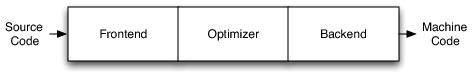
\includegraphics[width=\linewidth]{PICs/compiler_design.png}
	\caption{The stages of a three-pass compiler showing the way from source code to machine code}
	\label{fig:compiler_design}
\end{figure}

The biggest benefit from such an approach is that in theory it is simple to support different programming languages or machine architectures. If another language should be supported, this can be achieved by implementing a front-end for it while the optimizer and all existing back-ends just work without any big changes. The same applies for new target architectures, each requiring a new back-end, that supports every existing front-end out of the box. A good example for an open source compiler that supports several front-ends and back-ends is the GCC. But although the three-pass compiler design is well documented in various literature, in practice it is rather hard to uphold the separation all the time and several well-known open source projects did not do so. Due to that fact, \ac{LLVM} was created to unify and simplify the process of building languages and compilers. It shall also enhance the development of already existing languages. \cite{LLVM_ARCH}

One of the most important parts of \ac{LLVM} is its \ac{IR}. The \ac{LLVM} \ac{IR} is how code is represented in the compiler. The purpose of the \ac{IR} is to allow the compiler's optimizer to run mid-level transformations and analyses, while being a first class language with well-defined semantics on its own. The \ac{IR} in \ac{LLVM} serves as a perfect working environment for an optimizer, which is not constrained to any language or target specification. Beside the \ac{IR}, \ac{LLVM} uses a classical three-pass design. The front-end parsed the source code and generates \ac{LLVM} \ac{IR} from it, which is then handed to the optimizer for running several analysis and transformation passes. At the end all \ac{IR} code is passed to the back-end, where native machine code is generated from it. The implementation of \ac{LLVM}'s three-pass design can be seen in Figure \ref{fig:llvm_design}.

\begin{figure}[h!]
	\centering 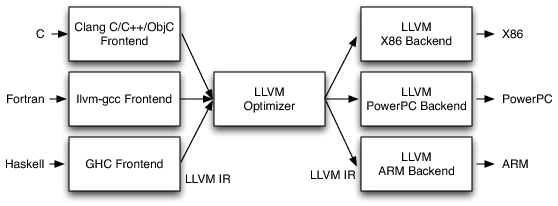
\includegraphics[width=\linewidth]{PICs/llvm_design.png}
	\caption{LLVM's implementation of the classical three-pass compiler design}
	\label{fig:llvm_design}
\end{figure}


\noindent
By using \ac{LLVM} during the compilation process, Rust gets all the benefits from already implemented optimizations in the \ac{LLVM} project. It is also responsible for the cross-platform abilities of \textit{rustc}, that is able to build binaries for different platforms specified by the compiler's toolchain.


\subsection{Rustup}

Rustup is a tool that helps installing the Rust toolchain. It allows the installation of different configurations and makes it possible to easily switch between several states of the Rust compiler. Beside being able to switch between nightly, beta and stable compiler versions, it is responsible for keeping them updated. It is currently able to run in all platforms, that are supported by Rust. With \textit{rustup} it is possible to install and manage several different Rust toolchains, managing them by a single set of tools. A toolchain in that context describes a single installation of \textit{rustc}.

Another important task of \textit{rustup} is the possibility to install additional targets for cross-compilation. Cross-compilation describes the process of generating compilation binaries for one machine (\textit{host platform}) on another, different one (\textit{build platform}). Because \textit{rustup} only installs the standard library binaries for the current platform, it is necessary to download them for the \textit{host platform} as well if the binaries shall be cross-compiled.

\subsection{Cargo}

Cargo is the package manager of the Rust programming language. Some of its features include downloading project dependencies, building the application, packaging crates and uploading them for distribution. It can be compared to package managers from other languages such as NPM from NodeJs or Nuget and C\# that are also capable of handling project dependencies in an automated fashion. But what makes Cargo rather unique and powerful are the capabilities it provides beside dependency management. It incorporates a build environment for Rust applications that is powerful and enhances the development process. Beside being able to invoke \textit{rustc} or a custom build script/tool, it is possible to test and benchmark a Rust application without any external tools. While other languages need to integrate that tools themselves , which often requires some amount of extra work, Cargo provides this important utilities out of the box.

Cargo is also the tool used to upload packages, or crates, to \textit{crates.io}, the Rust community;s package registry. Crates.io serves as a hub for many different libraries that can be used by any Rust application by simply depending onto them in the application's configuration file.

\section{Basic syntax}

Rust's syntax is quite similar to the one of C and even C++ in some parts. This section is going to showcase the its basic syntax based on examples to better understand the following concepts and code samples. It will also introduce some basics that are part of Rust's safety guarantees. 

\subsubsection{Variables, types \& mutability}

Because Rust is a statically typed programming language, every variable needs to have a distinct type specified at compile-time. As already mentioned the ability of type inference is not contradictory to statically typing. In Rust, the type of a variable can be annotated explicitly or inferred by the compiler. A variable declaration beginning with the \texttt{let} keyword do not require the programmer to specify the type, although it is not restricting an explicit declaration. Other variable declarations using \texttt{const} or \texttt{static} require a type to be annotated.\\

\begin{lstlisting}[caption={Variable bindings and mutability declarations in Rust}, label={lst:rust_var_bindings}, language=C]
	///
	/// Several variable bindings where both versions, type inference and type annotations, are showcased.
	/// The third binding will emit a warning because Rust sees that the literal exceeds the range of a 'u8'
	///
	let inferred  = 10;
	let annotated: u32 	= 42;
	let annotated_second: u8 = 1024;
	
	///
	/// Variable bindings with different mutability annotations
	///
	let immutable_var = 10;
	// immutable_var = 11 --> compilation error
	let mut mutable_var = 41;
	mutable_var = 42;
	
	///
	/// Rust does not allow implicit conversions between numerical types, 
	/// hence they have to be cast explicitly
	///
	let small_int: u32 = 100;
	let bigger_int: u64 = small_int as u64;
	
\end{lstlisting}

\noindent
As it can be seen in listing \ref{lst:rust_var_bindings}, Rust defaults all variable bindings to be immutable. Contradictory to C++, where immutable variables have to be marked as \texttt{const}, Rust requires the programmer to specify which variables are mutable by using the \texttt{mut} keyword.
Another situation where Rust prefers explicitness over implicitness is when casting between different types. Where in C++, numerical types can be implicitly converted to each other, Rust does not include such capabilities on purpose. If a type conversion shall be performed the programmer has to cast one type to the other by using either the \texttt{as} keyword, for a safe cast, or the \texttt{transmute} function, for an unsafe cast working quite similar to the \texttt{reinterpret\_cast} in C++.

\subsubsection{Pattern matching}

Another syntactical and functionally interesting feature of Rust are its pattern matching structures. Rust provides the \texttt{match} keyword, that works quite similar to a \texttt{switch} statement in C++, but is more powerful. 

\begin{lstlisting}[caption={Match statement in Rust, allowing for complex pattern matching in each arm}, label={lst:rust_match}, language=C]

	///
	/// 1) A match statement with range-based matches
	///
	let arr = [1, 2, 3, 4, 5, 6];
	
	match arr {
		[2, ..]  => { println!("Match if value at [0] is 2") },
		[1 .. 4] => { println!("Starting with 1 and ending with 4") },
		_ => { println!("Needed to handle every other case") }
	};
	
	///
	/// 2) A match statement with conditional patterns that returns from every arm
	///
	let x = 10;
	
	let res = match x {
		1 | 9 | 10 => { println!("Match if x is either 1 or 9"); true },
		_ => { println!("Match if x is 10"); true},
	};
	
	///
	/// 3) A match statement using destructuring
	///
	
	struct Data { 
		id: u32,
		amount: u64, 
	}
	
	let workload: Data = Data { id: 1, amount: 10 };
	
	match workload {
		Data { id: bind_one, amount: bind_two } => println!("Processing id: {} with amount: {}", bind_one, bind_two),
	}
	
\end{lstlisting}

\noindent
Listing \ref{lst:rust_match} shows several use cases of the match statement. The first match showcases the ability of complex patterns where the arms match only arrays that values are in a specific order. These complex patterns can be combined with conditional expressions, shown in the second match, making a pattern matching a powerful tool. In the third match, the expression of the first arm uses \textit{destructuring} in order to bind the fields of the structure to variables, that can be used in the body of that arm.

\section{Ownership system}

Regarding ownership Rust promises that the decision over a value's lifetime is up to the user and that the program, in spite of the given freedom, will never use a pointer to an already freed object (dangling pointer). While C++ allows for flexible lifetime decisions it cannot guarantee that the program does never hit a dangling pointer because it's the user's responsibility to ensure that no pointer to an already freed object is used.
Some highlevel languages such as Java or C\# solve the dangling pointer problem by introducing a garbage collector that controls when exactly objects are freed. This technique however also introduces an impact in performance.
To cope with this problem and to avoid garbage collection Rust came up with its own concept of ownership. In C++ and other languages it is said that an object 'owns' some other value that it points to and the owner therefore has control over the value's lifetime. In Rust this implicit ownership rule was turned to an explicit one and the language enforces that a value just has a single owner that controls its lifetime. As soon as the owner is freed, or dropped in Rust terminology, the owned value is dropped too. One example of Rust's ownership model is its \texttt{Box$<$T$>$} type that is a pointer to a value of type \textit{T} that is stored on the heap. When the \textit{Box} goes out of scope and is dropped, it frees the space it has allocated too, avoiding an otherwise introduce memory leak. \cite[Chapter 4. Ownership]{ProgrammingRust}
Whereas C++ also has constructs, called smart pointers, to express ownership, Rust's model comes without the overhead of storing additional meta data at runtime. Smart pointers have to store data for knowing when it is valid to drop the resource. Instead of this runtime overhead, Rust's system has to advantage of avoiding this overhead at all by moving the ownership checks to the compilation stage.

\subsection{Moves}

In C++, when a user assigns a variable to another or passes it to a function by-value, a copy of the value is created. Rust has chosen a different approach and instead of copying values, they are moved. When a move occurs,  the previous owner transfers ownership to the destination and gets uninitialized. The destination now controls the value's lifetime and becomes the new owner. Move semantics also exist in C++ and were introduced in the C++11 standard allowing the programmer to define move constructors and move assignment operators. \cite{CppMove} With the rule of using moves as the default behavior for assignment Rust can allow cheap assignments and keep the ownership clear as well. One trade-off the developer has to pay is that a copy now has to be requested explicitly. To do so in Rust one can implement either the \texttt{Copy} or \texttt{Clone} trait. What exactly a trait is and how they interact with other part of Rust is described in a later section. For now a trait can be though of as an extension, that can be implemented for other types, allowing them to be use by other code parts only knowing the trait's \ac{API}. The first one describes its implementor as trivially copyable by a plain \texttt{memcpy} where the second option requires the caller to invoke the \textit{clone} method that returns a new object. \cite[Chapter 4. Ownership]{ProgrammingRust}

\subsection{Borrows}

Beside owning pointers, such as a \texttt{Box$<$T$>$}, Rust also defines non-owning pointer types that are called \textit{references}. The major difference to owning-pointers is that a reference has no effect on the lifetime or ownership of the value it is pointing to. In Rust terminology the act of referencing a value is called \textit{$'$borrowing$'$} and the compiler enforces that no reference outlives its referent. There are two kinds of references in Rust -- \textit{shared} and \textit{mutable} ones. A shared reference allows to read the value but not modify it and there can be as many shared references as the programmer needs. A mutable reference however is allowed to be read and modified but no other reference is allowed to be active at the same time. This concept introduces the compile-time rule of either several readers or one writer which is essential to the memory safety of Rust. One thing that shall not stay unmentioned is a big difference between C++ and Rust references. While under the hood both are just addresses, Rust references are allowed to be reseated after initialization whereas C++ references just alias the object they have been initialized with and cannot be reassigned afterwards. \cite[Chapter 5. References]{ProgrammingRust}

\subsection{Lifetimes}
\blindtext
\section{Fearless concurrency}
\blindtext
\subsection{Data races}
\blindtext
\section{Traits}
\blindtext
\section{Modules}
\blindtext
\section{Generics}
\blindtext
\section{Hygienic macros}
\blindtext
\section{Missing or unstable features}
\blindtext
\subsection{Const generics}
\blindtext
\subsection{Placement-new functionality}
\blindtext